\subsection{Universal phenomena appear across settings and tasks}
\label{sec:reason-universal-behavior}


\begin{figure}
    \centering
    \hfill
    \begin{subfigure}{0.5\linewidth}
        \centering
        \includegraphics[width=\linewidth]{figs/universality/diffusion_arch_names.png}
        \caption{Universality across architectures}
    \end{subfigure}
    \hfill
    \begin{subfigure}{0.3\linewidth}
        \centering
        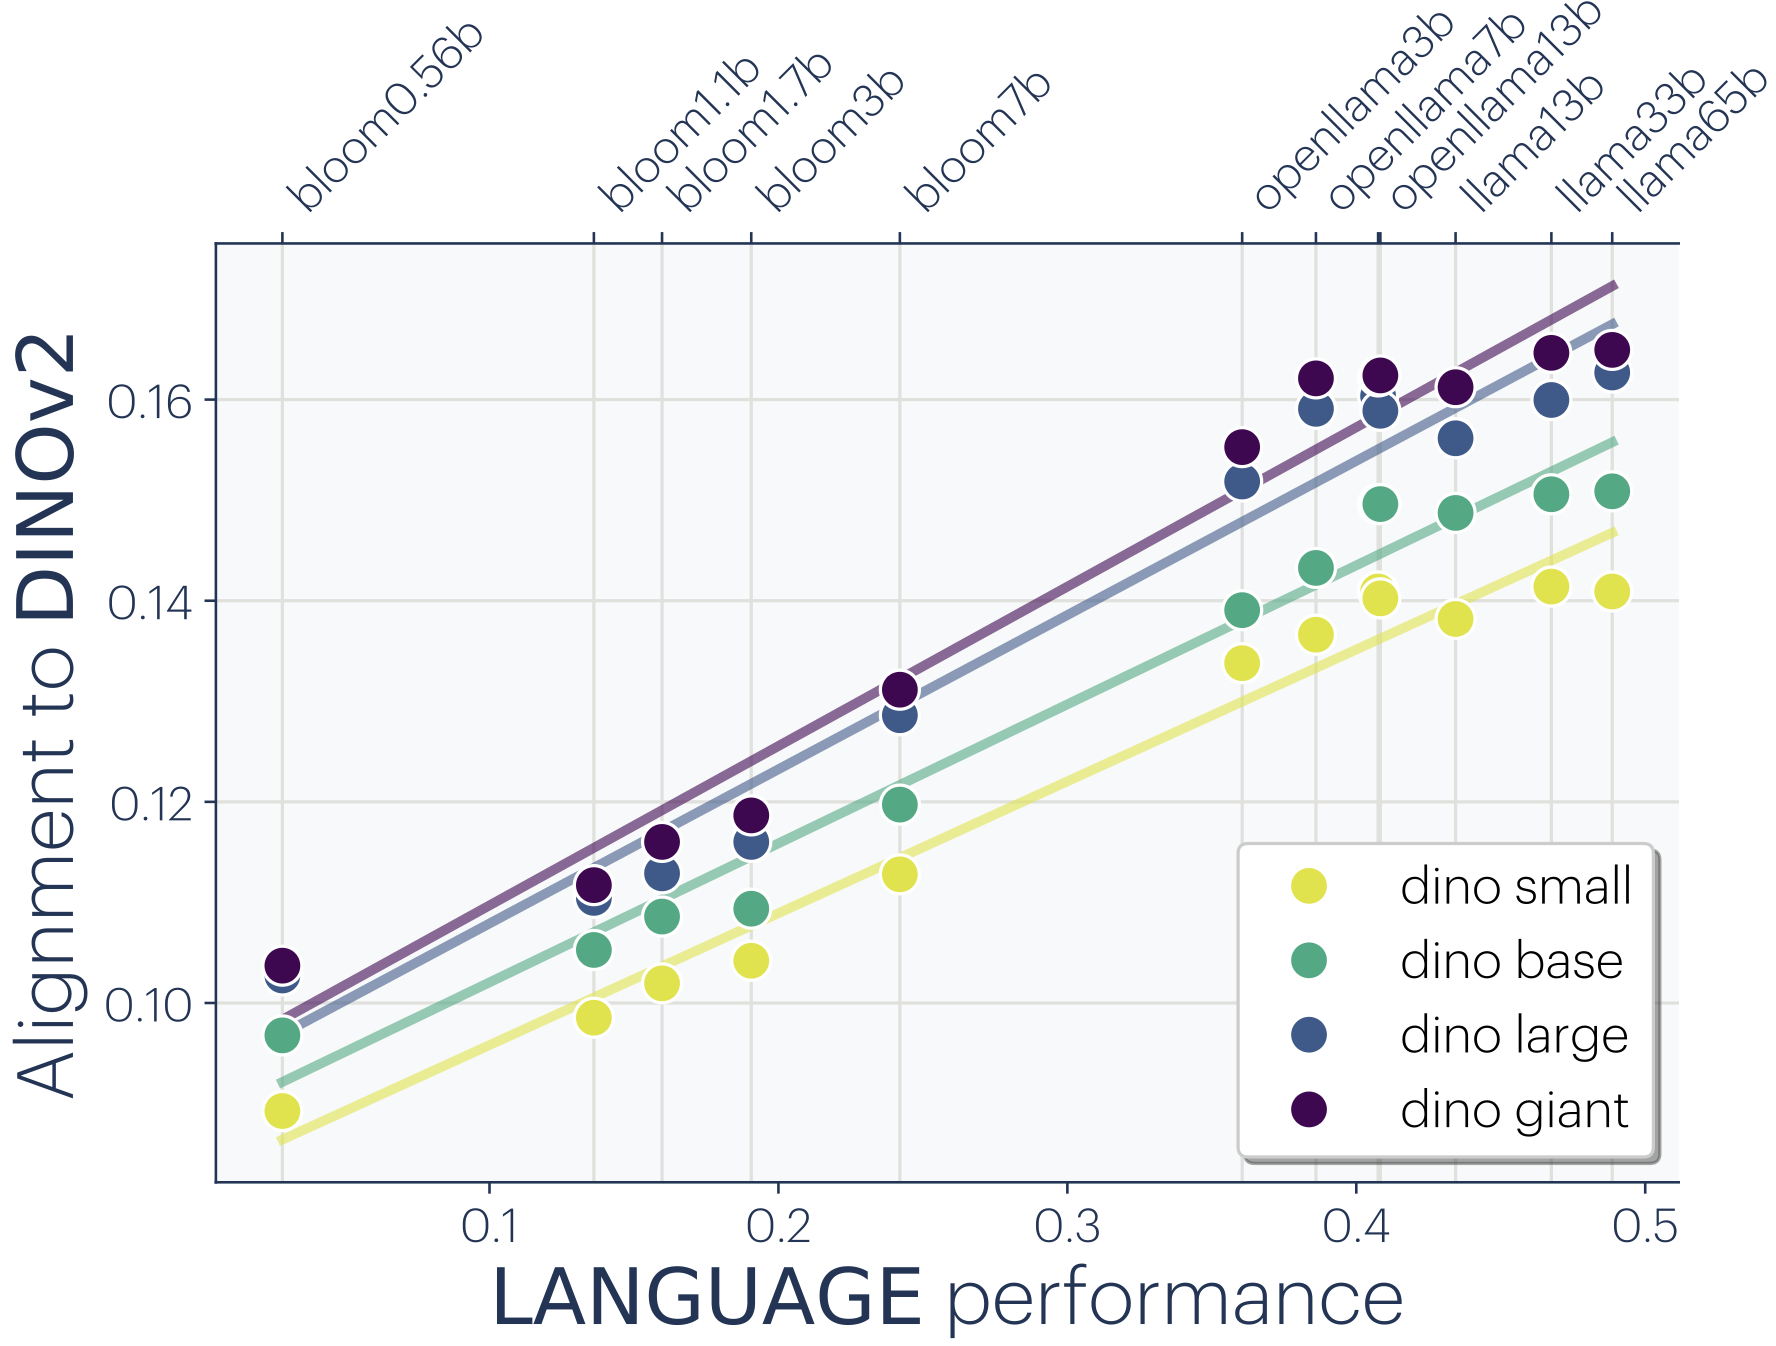
\includegraphics[width=\linewidth]{figs/universality/prh.png}
        \caption{Universality across data modalities}
    \end{subfigure}
    \hfill\null
    \caption{\textbf{Universality across architectures and data modalities.}
    (a):
    Different diffusion model architectures (from top to bottom: DDPM, a consistency model---both based on UNet---and U-ViT) converge to the same learned distribution and produce identical images when given the same input seed. Adapted from \citet{zhang2024emergence}
    (b): As language models performance (horizontal axis) increases, their internal representations become increasingly similar to that of vision models, and more so for larger models (from yellow to purple lines). Adapted from \citet{huh2024platonic}.
    }
    \label{fig:cka_width_cvg}
\end{figure}



Deep learning is not a single recipe followed exactly every time: different systems use very different architectures, datasets, training algorithms, and objectives, with ingredients combined in creative ways.
This versatility has enabled successes on many tasks and modalities including vision, language, speech, time series, protein sequences, and games, but the resulting model diversity makes it less clear how to approach the development of scientific theory.
Do these diverse settings share deep commonalities we might hope to capture scientifically?


Here, we review a growing body of evidence that there are indeed \textit{universal phenomena} at play in these diverse settings.
This is good news for theory: when many different complex systems exhibit the same universal behavior, it suggests that a simple underlying explanation may exist.
We highlight this universality through three different viewpoints: \textbf{(1)} different architectures
reach comparably good performance on many tasks; \textbf{(2)} different datasets share similar statistical properties; and \textbf{(3)} the learned representations and weights across different architectures and datasets are surprisingly alike.
This roughly echoes examples of universality in which disparate physical systems share deep commonalities %
or display similar behavior at large scales.%
\footnote{Universal behavior across physical systems can often be understood with the \textit{renormalization group,} a technique which formalizes the idea that, as one examines a system from a more and more zoomed-out perspective, most details ``wash out'' and only a handful of aggregate effects remain important. We note that another apt analogy for universality in deep learning, this one from biology, is \textit{convergent evolution}: species that ``solve similar problems'' tend to ``find similar solutions'' after many generations.}
We end by highlighting a few theoretical successes in modeling universal phenomena.







\paragraph{Universal inductive biases.}
Performance on a given task is often robust to variations in architectures, training algorithms, and objectives, in the sense that many alternate choices still lead to models that can solve the task.
A well-known example is the choice between convolutional networks and transformers in computer vision tasks, which after much debate have been shown to obtain similar performance when matching compute, data size, and training recipes \citep{liu2022convnet,smith2023convnets}.
In diffusion models, this similarity has been further shown to hold at the level of input-output mappings, with transformers and UNets generating near-identical images when fed with the same noise samples \citep{zhang2024emergence}, as shown in \cref{fig:cka_width_cvg}.
These results strongly indicate that different architectures share similar inductive biases despite their apparent differences.
As a partial explanation, recent work has shown that assuming inductive biases towards locality and adaptivity to geometric structures leads to accurate quantitative predictions about the behavior of diffusion generative models \citep{kadkhodaie2024generalization, kambanalytic, niedobatowards}.




\paragraph{Universal structure in data.}


The no-free-lunch theorem states that generalization on completely arbitrary data with a common learning strategy is not possible \citep{wolpert1996lack}.
Therefore, deep learning must rely on particular features of the data present across all datasets and modalities on which it succeeds.
For instance, many classes of images and audio signals share power-law spectral properties, sparsity patterns, and multiscale structures, and can be analyzed with general-purpose wavelet bases \citep{olshausen1996emergence,mallat1999wavelet}
A similar phenomenon in text data is the ubiquity of Zipf's law (word frequencies obey a power-law distribution) that holds over many natural and artificial languages \citep{li2002zipf,piantadosi2014zipf}. Hierarchical, compositional structure is also routinely used to model both images and text, which can sometimes be related through a common model \citep{cagnetta2024deep,sclocchi2025phase, cagnetta2025learning}. These shared statistical properties are a partial explanation for the ability of a single learning algorithm (say, a transformer trained with SGD) to tackle seemingly unrelated datasets, leaving only the finer-grained differences between them to be learned.




\paragraph{Universality in representations.} Going deeper in the internals of the network, it has been observed that representations learned by different networks can be similar across random initializations, widths, and architecture \citep{raghu2017svcca,kornblith2019similarity,bansal2021revisiting,huh2024platonic, moschella2022relative}. It has been shown that networks trained to solve different tasks learn similar representations across training datasets (ImageNet and Places-365, \citet{lenc2015understanding}), objectives (supervised or self-supervised, \citep{bansal2021revisiting}), and modalities (vision or language, \citep{huh2024platonic}). Furthermore, this similarity grows as model size and performance increase, hinting that neural activations converge towards a universal (``Platonic'') representation \citep{bansal2021revisiting, huh2024platonic}, as shown in \cref{fig:cka_width_cvg}.
In simplified settings such as random feature representations, this convergence is a consequence of the law of large numbers applied to the feature kernels \citep{rahimi2007random,guth2024rainbow}; in deep linear networks, it can be proven to arise from the implicit regularization of SGD~\citep{ziyin2025proof}; in more diverse settings, recent evidence suggests that the universality of representations may ultimately trace its origins to universal structure in data \citep{huh2024platonic,karkada2026symmetry}. Recent advances in {identifiability theory} \citep{hyvarinen2024identifiability} also have shown that representational convergence happens at the global optimum of unsupervised \citep{klindt2020towards}, self-supervised \citep{zimmermann2021contrastive} and supervised \citep{reizinger2024cross} objective functions under a suitable data generating process \citep{reizinger2025position}.
Several works have also shown empirically that this similarity can extend to the level of individual neurons \citep{li2015convergent,dravid2023rosetta,khosla2024privileged}. In some cases, similar representations have been found in both artificial neural networks and biological neural networks \citep{olshausen1996emergence, yamins2014performance, mcintosh2016deep}, though the extent of this correspondence remains controversial \citep{bowers2023deep}.
While a global trend towards similarity is emerging, it should be noted that the range of settings in which this convergence is observed, and its extent, are not fully known (see \cref{openquestion:comparing-models}).
In particular, recent work has shown that this apparent convergence to universal representations depends crucially on the chosen comparison metric across similarities \citep{groger2026revisiting}). A growing literature is devoted to understanding which representation similarity metrics one should choose in different circumstances \citep{sucholutsky2023getting,klabunde2025similarity} and highlighting the cases where they can be unified \citep{harvey2024duality,williams2024equivalence}.



If the mechanisms learned by large models are indeed universal, this is very encouraging for theory: behavior shared across \emph{many} systems should depend primarily on the features common to \emph{all} such systems, and thus admit a description simpler than any particular model in isolation.
Moreover, if the internal structure of trained neural networks primarily reflects the structure of data, then in studying neural networks we may ultimately be studying the structure of data and its generating processes (see \cref{openquestion:theory_for_real_data}).
In particular, since language data comes directly from humans, understanding its structure may teach us something new and fundamental about ourselves.
